\documentclass[12pt,a4paper]{jsarticle}

%\usepackage[latin1]{inputenc}
\usepackage{amsmath}
\usepackage{amsfonts}
\usepackage{amssymb}
\usepackage[dvipdfmx]{graphicx}
\usepackage{listings}

%ソースコード貼り付け設定
\usepackage{listings,jvlisting}
\usepackage{geometry}

\lstset{
  basicstyle={\ttfamily},
  identifierstyle={\small},
  commentstyle={\smallitshape},
  keywordstyle={\small\bfseries},
  ndkeywordstyle={\small},
  stringstyle={\small\ttfamily},
  frame={tb},
  breaklines=true,
  columns=[l]{fullflexible},
  xrightmargin=0zw,
  xleftmargin=3zw,
  numberstyle={\scriptsize},
  stepnumber=1,
  numbersep=1zw,
  lineskip=-0.5ex
}

\author{来代 勝胤}
\title{第3週課題}

\begin{document}
\maketitle
\thispagestyle{empty}
\clearpage
\addtocounter{page}{-1}

\newgeometry{left=15mm,right=15mm,top=15mm,bottom=20mm}
\begin{flushleft}
    {\large \textbf{【演習1】} \\
        Taylor-Green渦の二次元速度場の定常解$\left( t=\infty \right)$の
        $\textbf{u}\left(u,v\right)$を導出する.}\\
\end{flushleft}
$\left(x,y\right)$における,連続の式及びナビエ・ストークス方程式は,\\
以下の式(1),(2),(3)のように表せる.
\begin{eqnarray}
    \frac{\partial u}{\partial x} +
    \frac{\partial v}{\partial y} = 0
\end{eqnarray}\\
($x$方向)
\begin{eqnarray}
    -\frac{\partial u}{\partial t} =
    u\frac{\partial u}{\partial x} +
    v\frac{\partial u}{\partial y} +
    \frac{1}{\rho}\frac{\partial P}{\partial x}-
    \nu\nabla^2u
\end{eqnarray}\\
($y$方向)
\begin{eqnarray}
    -\frac{\partial v}{\partial t} =
    u\frac{\partial v}{\partial x} +
    v\frac{\partial v}{\partial y} +
    \frac{1}{\rho}\frac{\partial P}{\partial y}
    -\nu\nabla^2v
\end{eqnarray}\\
また,非圧縮性粘性流体における初期条件は以下の式(4),(5)のように与えられ,\\
このとき,式(6)が成立することが知られている.
\begin{eqnarray}
    u=A \cos ax \sin by
    \\
    v=B \sin ax \cos by
\end{eqnarray}
\begin{eqnarray}
    Aa+Bb=0
\end{eqnarray}
\begin{eqnarray}
    \frac{\partial u}{\partial t} =
    \frac{\partial v}{\partial t} = 0
\end{eqnarray}\\
以上の式(7)を式(2),(3)に用いて,\\
(2)を$x$で,(3)を$y$でそれぞれ偏微分すると,以下のようになる.
\begin{eqnarray}
    0 =
    \left(
    \frac{\partial u}{\partial x}
    \frac{\partial u}{\partial x}+
    u\frac{\partial^2 u}{\partial x^2}
    \right) +
    \left(
    \frac{\partial v}{\partial x}
    \frac{\partial u}{\partial y}+
    v\frac{\partial^2 u}{\partial x \partial y}
    \right) +
    \frac{1}{\rho}\frac{\partial^2 P}{\partial x^2}
    -\nu\nabla^2\frac{\partial u}{\partial x}
    \\
    0 =
    \left(
    \frac{\partial u}{\partial y}
    \frac{\partial v}{\partial x}+
    u\frac{\partial^2 v}{\partial x \partial y}
    \right) +
    \left(
    \frac{\partial v}{\partial y}
    \frac{\partial v}{\partial y}+
    v\frac{\partial^2 v}{\partial x^2}
    \right) +
    \frac{1}{\rho}\frac{\partial^2 P}{\partial y^2}
    -\nu\nabla^2\frac{\partial v}{\partial y}
\end{eqnarray}\\
ここで,式(8),(9)の和をとり,$-\frac{1}{\rho} \nabla^2P$について整理すると,
\begin{eqnarray}
    -\frac{1}{\rho} \nabla^2P
    =
    \left( \frac{\partial u}{\partial x}\right)^2
    +
    \left( \frac{\partial v}{\partial y}\right)^2
    +
    2\left(
    \frac{\partial u}{\partial y}
    \frac{\partial v}{\partial x}
    \right)
\end{eqnarray}\\
このとき,$\frac{\partial u}{\partial x}$,
$\frac{\partial v}{\partial y}$,
$\frac{\partial u}{\partial y}$,
$\frac{\partial v}{\partial x}$はそれぞれ以下のように表せる.
\begin{eqnarray}
    \frac{\partial u}{\partial x}
    =&
    -Aa \sin{ax} \sin{by}
    \\
    \frac{\partial u}{\partial y}
    =&
    \quad Ab \cos{ax} \cos{by}
    \\
    \frac{\partial v}{\partial x}
    =&
    \quad Ba \cos{ax} \cos{by}
    \\
    \frac{\partial v}{\partial y}
    =&
    -Bb \sin{ax} \sin{by}
\end{eqnarray}\\
以上の計算結果を用いて,式(10)に代入して整理すると,
\begin{eqnarray}
    \frac{1}{\rho} \nabla^2P
    =
    -A^2a^2
    \left(
    \cos{2ax}
    +
    \cos {2by}
    \right)
\end{eqnarray}\\
積分すると,
\begin{eqnarray}
    \frac{P}{\rho}
    =
    -\frac{1}{4}A^2a^2
    \left(
    \frac{1}{a^2} \cos{2ax}
    +
    \frac{1}{b^2} \cos{2by}
    \right)
\end{eqnarray}\\
また,式(2),(3)において,$\frac{1}{\rho}\frac{\partial P}{\partial x}$,
$\frac{1}{\rho}\frac{\partial P}{\partial y}$,$ \nabla^2u$,$\nabla^2v$
はそれぞれ以下のように表せる.
\begin{eqnarray}
    \frac{1}{\rho}
    \frac{\partial P}{\partial x}
    =
    \frac{A^2a^2}{2a}\sin {2ax}
    \\
    \frac{1}{\rho}
    \frac{\partial P}{\partial y}
    =
    \frac{A^2a^2}{2b}\sin {2ay}
\end{eqnarray}
\begin{eqnarray}
    \nabla^2u
    =&
    -A
    \left(
    a^2+b^2
    \right)
    \cos{ax}\sin{by}
    \\
    \nabla^2v
    =&
    -B
    \left(
    a^2+b^2
    \right)
    \sin{ax}\cos{by}
\end{eqnarray}\\
以上の式(17)〜(20)の計算結果及び(11)〜(14)を用いて(2),(3)に代入する.\\
その後,$\frac{\partial u}{\partial t}$,$\frac{\partial v}{\partial t}$について整理すると,
以下の式を得ることができる.
\begin{eqnarray}
    \frac{\partial u}{\partial t}
    =
    -\nu \theta A \cos{ax} \sin{by}
\end{eqnarray}
\begin{eqnarray}
    \frac{\partial v}{\partial t}
    =
    -\nu \theta B \sin{ax} \cos{by}
\end{eqnarray}
\\
ここで,$\theta=a^2+b^2$ とする.\\
式(21)および(22)を積分して,
\begin{eqnarray}
    u=-\nu \theta A t \cos{ax} \sin{by}+C_1
    \\
    v=-\nu \theta B t \sin{ax} \cos{by}+C_2
\end{eqnarray}
\\
ここで,式(4),式(5)から,$C_1$および$C_2$は,以下のように表せるので,
\begin{eqnarray}
    C_1=A \cos ax \sin by
    \\
    C_2=B \sin ax \cos by
\end{eqnarray}
\\
したがって,$u$,$v$はそれぞれ以下のように表すことができる.
\begin{eqnarray}
    u
    =
    \left(
    1-\nu \theta t
    \right)
    A \cos ax \sin by
    \\
    v
    =
    \left(
    1-\nu \theta t
    \right)
    B \sin ax \cos by
\end{eqnarray}\\
同様の手順で計算を行い,$u$,$v$を求めると,以下の式(43),(44)のようになる.\\ \\
● $u$,$v$をそれぞれ$x$,$y$で偏微分する.
\begin{eqnarray}
    \frac{\partial u}{\partial x}
    =&
    \left(
    1-\nu \theta A t
    \right)
    a \sin{ax} \sin{by}
    \\
    \frac{\partial u}{\partial y}
    =&
    \left(
    1-\nu \theta A t
    \right)
    b \cos{ax} \cos{by}
    \\
    \frac{\partial v}{\partial x}
    =&
    \left(
    1-\nu \theta B t
    \right)
    a \cos{ax} \cos{by}
    \\
    \frac{\partial v}{\partial y}
    =&
    \left(
    1-\nu \theta B t
    \right)
    b \sin{ax} \sin{by}
\end{eqnarray}
\\
● 式(10)に代入して整理し,積分する.
\begin{eqnarray}
    \frac{1}{\rho} \nabla^2P
    =
    A^2a^2
    \left(
    \cos{2ax}
    +
    \cos {2by}
    \right)
    \nu^2 \theta^2 t^2
\end{eqnarray}
\begin{eqnarray}
    \frac{P}{\rho}
    =
    \frac{1}{4}A^2a^2
    \left(
    \frac{1}{a^2} \cos{2ax}
    +
    \frac{1}{b^2} \cos{2by}
    \right)
    \nu^2 \theta^2 t^2
\end{eqnarray}
\\
●  $\frac{1}{\rho}\frac{\partial P}{\partial x}$,
$\frac{1}{\rho}\frac{\partial P}{\partial y}$,$ \nabla^2u$,$\nabla^2v$
をそれぞれ算出する.
\begin{eqnarray}
    \frac{1}{\rho}
    \frac{\partial P}{\partial x}
    =
    \frac{A^2a^2}{2a}\sin {2ax}
    \,\nu^2 \theta^2 t^2
    \\
    \frac{1}{\rho}
    \frac{\partial P}{\partial y}
    =
    \frac{A^2a^2}{2b}\sin {2ay}
    \,\nu^2 \theta^2 t^2
\end{eqnarray}
\\
● 式(37),(38)をそれぞれ積分する.
\begin{eqnarray}
    \nabla^2u
    =&
    A
    \left(
    a^2+b^2
    \right)
    \cos{ax}\sin{by}
    \,\nu^2 \theta^2 t^2
    \\
    \nabla^2v
    =&
    B
    \left(
    a^2+b^2
    \right)
    \sin{ax}\cos{by}
    \,\nu^2 \theta^2 t^2
\end{eqnarray}\\
● 式(27),(28)を用いて,積分定数$C_3$及び$C_4$を計算する.
\begin{eqnarray}
    u=\frac{1}{2}\,\nu^2 \theta^2 A t^2 \cos{ax} \sin{by}+C_3
    \\
    v=
    \frac{1}{2}\,\nu^2 \theta^2 B t^2 \sin{ax} \cos{by}+C_4
\end{eqnarray}
\begin{eqnarray}
    C_3
    =
    \left(
    1-\nu \theta t
    \right)
    A \cos ax \sin by
    \\
    C_4
    =
    \left(
    1-\nu \theta t
    \right)
    B \sin ax \cos by
\end{eqnarray}
\begin{eqnarray}
    u
    =
    \left(
    1-\nu \theta t + \frac{1}{2}\,\nu^2 \theta^2 t^2
    \right)
    A \cos ax \sin by
    \\
    v
    =
    \left(
    1-\nu \theta t + \frac{1}{2}\,\nu^2 \theta^2 t^2
    \right)
    B \sin ax \cos by
\end{eqnarray}\\
\newpage
ここで,$e^{- \nu \theta t}$が,指数関数の
テイラー展開から以下のように表せることから,
\begin{eqnarray}
    e^{- \nu \theta t}
    =
    1
    -
    \nu \theta t
    +
    \frac{1}{2}\,\nu^2 \theta^2 t^2
    -
    \frac{1}{3!}\,\nu^3 \theta^3 t^3
    +
    \dots
    +
    \left(
    -1
    \right)^{n-1}
    \frac{1}{
        \left(
        n-1
        \right)!
    }
    \left(
    \nu \theta t
    \right)^{n-1}
\end{eqnarray}
\\
$u$および$v$が計算を繰り返し,n回目の計算を終えたとき,\\
式(4),(5),(27),(28),(43),(44)を用いて以下のように表すことができると考えられる.
\begin{eqnarray}
    \begin{aligned}
        u_n
        = &
        \left(
        1
        -
        \nu \theta t
        +
        \frac{1}{2}\,\nu^2 \theta^2 t^2
        -
        \frac{1}{3!}\,\nu^3 \theta^3 t^3
        +
        \dots
        +
        \left(
            -1
            \right)^{n-1}
        \frac{1}{
                \left(
                n-1
                \right)!
            }
        \left(
            \nu \theta t
            \right)^{n-1}
        \right)
        \\
          & A \cos ax \sin by
        \\
        = &
        e^{- \nu \theta t} A \cos ax \sin by
        \\
        = &
        e^{- \nu
                \left(
                a^2 + b^2
                \right) t}
        A \cos ax \sin by
    \end{aligned}
\end{eqnarray}
\begin{eqnarray}
    \begin{aligned}
        v_n
        = &
        \left(
        1
        -
        \nu \theta t
        +
        \frac{1}{2}\,\nu^2 \theta^2 t^2
        -
        \frac{1}{3!}\,\nu^3 \theta^3 t^3
        +
        \dots
        +
        \left(
            -1
            \right)^{n-1}
        \frac{1}{
                \left(
                n-1
                \right)!
            }
        \left(
            \nu \theta t
            \right)^{n-1}
        \right)
        \\
          & B \sin ax \cos by
        \\
        = &
        e^{- \nu \theta t} B \sin ax \cos by
        \\
        = &
        e^{- \nu
                \left(
                a^2 +b^2
                \right)
                t} B \sin ax \cos by
    \end{aligned}
\end{eqnarray}
\\
したがって,$u$,$v$はそれぞれ以下のように表すことができる.
\begin{eqnarray}
    \begin{cases}
        {u = e^{- \nu
                    \left(
                    a^2 + b^2
                    \right) t}
            A \cos ax \sin by}
        \\
        {v =  e^{- \nu
                \left(
                a^2 +b^2
                \right)
                t} B \sin ax \cos by}
    \end{cases}
\end{eqnarray}
\\
ここで,式(6)の条件から,$A=a=b=1$,$B=-1$とすると,
\\
$u$,$v$はそれぞれ以下のように表される.
\begin{eqnarray}
    \begin{cases}
        {u = e^{- 2 \nu t}
            \cos x \sin y}
        \\
        {v = -e^{- 2 \nu t}
        \sin x \cos y}
    \end{cases}
\end{eqnarray}
\\
\begin{flushleft}
    {\large \textbf{【演習2】}\\
        渦度場$\omega_z$を導出する.} \\
\end{flushleft}
式(49)を用いて2次元ベクトル場における渦度$\omega_z$は以下の式(50)のように表される.\\
それを用いて$\omega_z$を計算すると,式(53)のように表すことができる.
\begin{eqnarray}
    \omega_z
    =
    \frac{\partial v}{\partial x}
    -
    \frac{\partial u}{\partial y}
\end{eqnarray}
\begin{eqnarray}
    \frac{\partial v}{\partial x}
    &=
    -e^{- 2 \nu t}\cos{x} \cos{y}
    \\
    \frac{\partial u}{\partial y}
    &=
    e^{- 2 \nu t}\cos{x} \cos{y}
\end{eqnarray}
\begin{eqnarray}
    \omega_z
    =
    -2 e^{- 2 \nu t}
    \cos{ax} \cos{by}
\end{eqnarray}\\
\newgeometry{left=10mm,right=10mm,top=15mm,bottom=20mm}
\begin{flushleft}
    {\large \textbf{【演習3】}\\
        プログラム} \\
\end{flushleft}
\small
\begin{lstlisting}
/******************************************************************************
PROGRAM NAME : practice_3
AUTHER : Masatsugu Kitadai
DATE : 1/4/2021
Think a Bit , Code a Bit , Test a Bit
******************************************************************************/
#include <stdio.h>
#include <stdlib.h>
#include <math.h>
#include <sys/stat.h>
#define x_grid 31                                        // number of grids in x direction
#define y_grid 31                                        // number of grids in y direction
const char grid_space = 1;                               // grid width
const char *output_data_file = "2dvec_vortex000001.dat"; // name of output file
double u[x_grid][y_grid];                                // u vector array
double v[x_grid][y_grid];                                // v vector array
double U[x_grid][y_grid];                                // absolute vector array
double omega[x_grid][y_grid];                            // vorticity array

double a[x_grid][y_grid];
double b[x_grid][y_grid];
double c[x_grid][y_grid];
double d[x_grid][y_grid];

FILE *output_file; // pointer for output file

const char *xxlabel = "{/Times-New-Roman:Italic=20 x} [pixel]";
const char *yylabel = "{/Times-New-Roman:Italic=20 y} [pixel]";
const char *cb_label = "{/Symbol:Italic=20 w}_{/Times-New-Roman:Italic=20 z} [sec]"; ///color bar range min

const double v_r = 1.0; ///magnified ratio for vector length

const int x_min = 0;   ///x range min
const int x_max = 30;  ///x range max
const int y_min = 0;   ///y range min
const int y_max = 30;  ///y range max
const int cb_min = -2; ///color bar range min
const int cb_max = 2;  ///color bar range max

const char *read_file_dir = "01_plot_vec_vortex";
const char *read_file_header = "2dvec_vortex";
const char *write_file_dir = "02_splot_2dvec_vortex_map";
const char *write_file_header = "2dvec_vortex_map";

//Graph parameters for GNU
char read_file[100];
void graph_GNU(); //png & eps
FILE *gp;         //gnuplot
FILE *infile;

int moveFile(const char *srcPath, const char *destPath)
{
        return !rename(srcPath, destPath);
    }

/*********************************
MAIN
*********************************/
double main()
{
int i, j;
double PI = 4.0 * atan(1.0);

// preparing for output file
output_file = fopen(output_data_file, "w");

// Array initialization
for (i = 0; i < x_grid; i++)
{
        for (j = 0; j < y_grid; j++)
        {
                u[i][j] = 0;
                v[i][j] = 0;
                U[i][j] = 0;
                omega[i][j] = 0;
            }
    }

// Calc.2D velocity vector and absolute value of velocity field, vorticity field

for (i = 0; i < x_grid; i++)
{
        for (j = 0; j < y_grid; j++)
        {
                //  velocity vector field and absolute value of vector
                u[i][j] = cos(2.0 * PI / x_grid * i) * sin(2.0 * PI / y_grid * j);
                v[i][j] = -sin(2.0 * PI / x_grid * i) * cos(2.0 * PI / y_grid * j);
                U[i][j] = sqrt(u[i][j] * u[i][j] + v[i][j] * v[i][j]);

                // value of vorticity field
                omega[i][j] = -2 * cos(2.0 * PI / x_grid * i) * cos(2.0 * PI / y_grid * j);

                fprintf(output_file, "%d\t%d\t%3lf\t%.3lf\t%.3lf\t%3lf\n",
                i * grid_space, j * grid_space, omega[i][j], u[i][j], v[i][j], U[i][j]);

                //Caution : just line breaking for printing this document

                /*
                printf("%d\t,%d\t,%.3lf\t,%.3lf\t,%.3lf\t,%.3lf\n",
                i * grid_space, j * grid_space, omega[i][j], u[i][j], v[i][j], U[i][j]);
                */
            }
        fprintf(output_file, "\n");
        //printf("\n");
    }

fclose(output_file);

mode_t mode = S_IRWXU | S_IRGRP | S_IXGRP | S_IROTH | S_IXOTH;
mkdir(read_file_dir, mode);
mkdir(write_file_dir, mode);

// transfer the result file to the specified folder

if (moveFile("2dvec_vortex000001.dat", "01_plot_vec_vortex/2dvec_vortex000001.dat"))
{
        puts("transferred the file");
    }
else
    {
        puts("cannot transferred");
    }

int k = 0;
int UP = 0;
while (UP == 0)
{
k++;
sprintf(read_file, "%s//%s%06d.dat", read_file_dir, read_file_header, k);
printf("%s//%s%06d.dat\n", read_file_dir, read_file_header, k);
infile = fopen(read_file, "rb");

if (infile == NULL)
{
        printf("break!\n");
        break;
    }

fclose(infile);

if ((gp = popen("gnuplot", "w")) == NULL)
{
        printf("gnuplot is not here!\n");
        exit(0);
    }

//PNG image
fprintf(gp, "set terminal pngcairo enhanced font 'Times New Roman,15' \n");
fprintf(gp, "set output '%s//%s%06d.png'\n", write_file_dir, write_file_header, k);
fprintf(gp, "set multiplot\n");     // <steps in scan>,<steps between scans>
fprintf(gp, "unset key\n");         // <steps in scan>,<steps between scans>
fprintf(gp, "set size ratio -1\n"); // <steps in scan>,<steps between scans>

fprintf(gp, "set lmargin screen 0.15\n"); // <steps in scan>,<steps between scans>
fprintf(gp, "set rmargin screen 0.85\n"); // <steps in scan>,<steps between scans>
fprintf(gp, "set tmargin screen 0.85\n"); // <steps in scan>,<steps between scans>
fprintf(gp, "set bmargin screen 0.15\n"); // <steps in scan>,<steps between scans>

fprintf(gp, "set xrange [%d:%d]\n", x_min, x_max);       // <steps in scan>,<steps between scans>
fprintf(gp, "set xlabel '%s'offset 0.0,0.5\n", xxlabel); // <steps in scan>,<steps between scans>
fprintf(gp, "set yrange [%d:%d]\n", y_min, y_max);       // <steps in scan>,<steps between scans>
fprintf(gp, "set ylabel '%s'offset 0.5,0.0\n", yylabel); // <steps in scan>,<steps between scans>

fprintf(gp, "set cblabel '%s'offset 0.0,0.0\n", cb_label);
fprintf(gp, "set cbrange['%d':'%d']\n", cb_min, cb_max);
fprintf(gp, "set colorbox vertical user origin 0.8, 0.2 size 0.025,0.6\n");
fprintf(gp, "set palette rgbformulae 22,13,-31\n");

fprintf(gp, "set pm3d map\n"); // <steps in scan>,<steps between scans>
fprintf(gp, "splot '%s//%s%06d.dat' using 2:1:3 with pm3d, '%s//%s%06d.dat' using 2:1:($1*0.0):(%lf*$5):(%lf*$4):($1*0.0) with vectors head filled lt 2 lc 'black' \n", read_file_dir, read_file_header, k, read_file_dir, read_file_header, k, v_r, v_r);

fflush(gp); //Clean up Data

fprintf(gp, "exit\n"); // Quit gnuplot

pclose(gp);
}

return (0);
}
\end{lstlisting}

\newpage

\begin{center}
    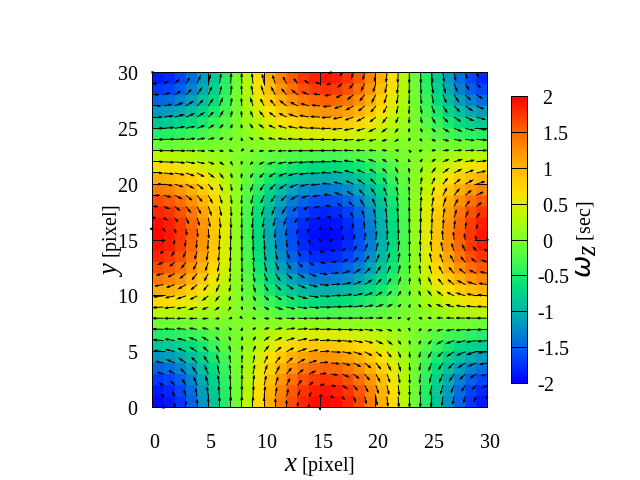
\includegraphics[width=150mm]{2dvec_vortex_map000001.png}
    \large
    \\ 図1 gnuplotで作図した速度場ベクトル及び渦度場
\end{center}

\end{document}